
We monitored the accuracy of our embeddings over the course of training our CNN. The validation set is a dataset of 1000 triplets such that 100 triplets are created from each of the 10 validation videos. After the end of training, 736/1000 samples fulfilled the triplet constraint. 930/1000 fulfilled the contrained without the added margin. I.e. $\norm{x_a - x_p} < \norm{x_a - x_n}$.

For comparison after 10 epochs of training the values were 467/1000 with margin and 894/1000 without the margin.

{
    \label{example-snap}
    \centering
    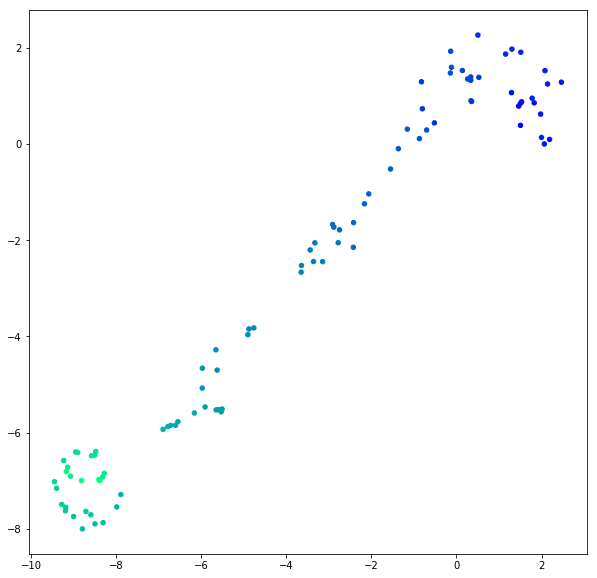
\includegraphics[width=8cm]{t-sne-trajectory.png}
    \captionof{figure}{A t-SNE plot of a validation trajectory. Perplexity 30, learning rate 200 and 1000 iterations. The color goes from blue to cyan as a function of the frame indices.}
    \vspace{0.5cm}
}

The t-SNE plot of a validation trajectory suggests that the network has learned a meaningful and well-behaved embedding of the video frames. Embeddings of frames that are close to each other in the video are close to each other in the dimentionality reduced regime.


